\documentclass[11pt,a4paper]{report}

\usepackage[utf8]{inputenc}
\usepackage[T1]{fontenc}
\usepackage{lmodern}
\usepackage{graphicx}
\usepackage{geometry}
\usepackage{xcolor}
\usepackage{setspace}
\usepackage{fancyhdr}
\usepackage{tocloft}
\usepackage[hidelinks]{hyperref}
\usepackage{titlesec}
\usepackage{booktabs}
\usepackage[table]{xcolor}
\usepackage{longtable}
\usepackage{array}
\usepackage{caption}
\usepackage{float}
\usepackage{amsmath, amssymb, bm}
\usepackage{pgfplots}
\pgfplotsset{compat=1.18}
\usepackage{tikz}
\usetikzlibrary{calc, arrows.meta, positioning}
\usepackage{pdflscape}
\usepackage{eso-pic}
\usepackage{lastpage} 
\usepackage{tcolorbox}
\usepackage{listings}
\usepackage{xcolor}

\lstset{
  basicstyle=\ttfamily\small,
  breaklines=true,
  breakatwhitespace=true,
  columns=fullflexible
}



% \usepackage{pdflscape}   % <-- già caricato sopra, puoi lasciare commentato
% \usepackage{caption}     % <-- già caricato sopra, puoi lasciare commentato


\geometry{top=2.5cm, bottom=2.5cm, left=3cm, right=3cm}
\setlength{\parskip}{1em}
\setlength{\parindent}{0pt}

\definecolor{bocconiblue}{RGB}{0,45,114}
\colorlet{rowlight}{bocconiblue!10}

% === Colonna laterale azzurra su ogni pagina ===
\AddToShipoutPictureBG{%
  \begin{tikzpicture}[remember picture, overlay]
    \fill[bocconiblue!10] (current page.north west) rectangle ++(1.2cm,-\paperheight);
  \end{tikzpicture}%
}

\pagestyle{fancy}
\fancyhf{}
\fancyfoot[C]{\thepage}
\renewcommand{\headrulewidth}{0pt}

% =========================
%   TITOLO / AUTORI
% =========================
\title{
\textbf{EICTA Third Project Delivery}\\[6pt]
\large Technical Report on the Web Application
}

\author{
Group Number: 4 \\[6pt]
Academic Year 2025--2026 \\[12pt]
\textbf{Authors:}\\[4pt]
Annalaura Catalfo --- Bocconi: 3200742 --- PoliMI: 11182469\\
Guendalina Nardi --- Bocconi: 3376114 --- PoliMI: 11179726\\
Giacomo Nigro --- Bocconi: 3186734 --- PoliMI: 11182213\\
Sofia Varotto --- Bocconi: 3221388 --- PoliMI: 11182433
}

\date{} % niente data

% =========================
%   INIZIO DOCUMENTO
% =========================
\begin{document}
\begin{titlepage}
\centering


\begin{tabular}{c@{\hspace{1cm}}|@{\hspace{1cm}}c}
\includegraphics[height=2.6cm]{ba.png} &
\includegraphics[height=2.6cm]{poli.png}
\end{tabular}

\vspace{7cm}

{\LARGE\bfseries EICTA Second Project Delivery -- Neo4j and BPMN\par}

\vspace{7cm}
{\Large Group Number: 4}\\[0.3cm]
{\Large Academic Year 2025--2026}

\vspace{1cm}

\begin{minipage}{0.85\textwidth}
\raggedleft
\centering
\textbf{Authors:}\\[0.5em]

Annalaura Catalfo — Bocconi: 3200742 — PoliMI: 11182469\\
Guendalina Nardi - Bocconi: 3376114 — PoliMI: 11179726\\
Giacomo Nigro — Bocconi: 3186734 — PoliMI: 11182213\\
Sofia Varotto — Bocconi: 3221388 — PoliMI: 11182433
\end{minipage}

\vfill

\end{titlepage}

% =========================
%   INDICE
% =========================
\pagenumbering{roman}
\begingroup
\pagestyle{empty}
\tableofcontents
\endgroup
\clearpage
\pagenumbering{arabic}

\newpage
\chapter{Mongo  Festival Database}
\section{Modeling the Festival collection}

In our MongoDB design we use a single collection, named \texttt{Festival}, which represents the main entity of the domain. Each document in the collection acts as a root document and corresponds to a specific edition of a festival.\\
Within each root document, we embedded all entities connected to Festival through 1:N relationships: \texttt{Stage, Performance, Artist, Stand, Product}, and \texttt{Ticket}, modeling them as nested sub-documents.

The document structure mirrors the domain hierarchy: the \texttt{Festival} document contains the arrays of \texttt{Stages, Stands}, and \texttt{Tickets}; each \texttt{Stage} contains its \texttt{Performances}, each \texttt{Performance} contains its \texttt{Artists}, and each \texttt{Stand} contains its \texttt{Products}.\\
This layout allows a full festival edition to be represented within a single JSON document, avoiding joins and simplifying queries. It also fully satisfies the assignment requirement of using a single collection with multiple non-empty sub-document arrays.

\section{Cardinalities and nesting}

In the original ER model, all relationships involving the Festival entity were of type 1:N (Festival→Stage, Stage→Performance, Performance→Artist, Festival→Stand, Stand→Product, Festival→Ticket). According to standard document-modeling principles, such relationships are naturally represented using arrays of sub-documents.

The presence of hierarchical chains, such as Festival → Stage → Performance → Artist and Festival → Stand → Product, requires using multi-level nesting. This preserves the structure and semantics of the domain and makes the relationships explicit: for example, it is always clear which Stage a Performance belongs to or which Products are associated with a specific Stand, without relying on references or join-like mechanisms.

\section{Modeling ISA hierarchies}

The ER model included two ISA hierarchies: ``Product $\rightarrow$ Food, Drink, Merchandise'' and ``Artist $\rightarrow$ Solo\_Musician, Band'', both Total Exclusive.
In MongoDB, each ISA was collapsed into a single unified sub-document, using a discriminator field and, where appropriate, optional attributes.

Products are represented by a single \texttt{Product} sub-document containing a \texttt{Category} discriminator field and optional attributes such as \texttt{IsVegetarian} (for Food) or \texttt{Alcoholic} (for Drink).\\
Artists are represented by a single \texttt{Artist} sub-document with a \texttt{Type} discriminator field (\texttt{"solo"} or \texttt{"band"}), without optional fields since both specializations share the same attributes.

This approach aligns with NoSQL best practices for handling exclusive ISA hierarchies: it ensures a uniform, compact, and easily queryable schema, avoids structural redundancy, and simplifies the overall nesting strategy in the document model.

\section{Document Structure: Attributes, Types and Containment Hierarchy}
\subsection{Festival (root document)}

The \texttt{Festival} document represents the main entity and is the top level of the structure. It contains all information of the festival edition and serves as a container for all hierarchically related sub-documents.


\lstset{
    basicstyle=\ttfamily\small,
    keywordstyle=\color{blue}\bfseries,
    stringstyle=\color{teal},
    commentstyle=\color{gray},
    numbers=left,
    numberstyle=\tiny\color{gray},
    stepnumber=1,
    numbersep=8pt,
    showstringspaces=false,
    breaklines=true,
    numbers=none,
    frame=none,            % <-- RIMUOVE IL RIQUADRO
    backgroundcolor=\color{white},
}


\begin{lstlisting}
{
    "_id": ObjectId,
    "FestivalId": String,
    "Name": String,
    "Location": String,
    "Country": String,
    "Date": {
        "StartDate": String,   // ISO date "YYYY-MM-DD"
        "EndDate": String
    },
    "Description": String,
    "Genres": [String],
    "Stages": [Stage],
    "Stands": [Stand],
    "Tickets": [Ticket]
}
\end{lstlisting}

\subsubsection{Attributes and Types:}

\begin{itemize}
    \item FestivalId : String
    \item Name : String
    \item Location : String
    \item Country : String
    \item Date.StartDate : String (ISO date “YYYY-MM-DD”)
    \item Date.EndDate : String (ISO date “YYYY-MM-DD”)
    \item Description : String
    \item Genres : Array<String>
    \item Stages : Array<Stage>
    \item Stands : Array<Stand>
    \item Tickets : Array<Ticket>
    
\end{itemize}

\subsection{Stage (sub-document of Festival)}
Each festival contains one or more stages, and each stage hosts a list of performances.

\subsubsection{Attributes and Types:}

\begin{itemize}
    \item StageId : String
    \item Name : String
    \item Capacity : Number
    \item Performances : Array<Performance>
\end{itemize}

\subsection{Performance (sub-document of Stage)}

Each stage contains a set of performances, each with its own schedule and associated artists.

\subsubsection{Attributes and Types:}
\begin{itemize}
    \item PerformanceId : String
    \item Title : String
    \item Day : Number
    \item StartTime : String (ISO datetime “YYYY-MM-DDTHH:MM:SS”)
    \item EndTime : String (ISO datetime)
    \item Artists : Array<Artist>
\end{itemize}

\subsection{Artist (sub-document of Performance)}
Each performance includes multiple artists or bands. The “Solo/Band” ISA hierarchy is handled through a discriminator.

\subsubsection{Attributes and Types:}
\begin{itemize}
    \item ArtistId : String
    \item Name : String
    \item Type : String (“solo” | “band”)
    \item Country : String
    \item Genre : String
\end{itemize}

\subsection{Stand (sub-document of Festival)}
Each festival includes several stands dedicated to food, drinks, or merchandising.

\subsubsection{Attributes and Types:}

\begin{itemize}
    \item StandId : String
    \item Name : String
    \item Type : String (“food”, “drink”, “merch”)
    \item Sponsor : String (optional)
    \item Products : Array<Product>
\end{itemize}

\subsection{Product (sub-document of Stand)}
Stands sell products of different types (Food/Drink/Merchandise). The ISA hierarchy is handled through a discriminator and optional fields.

\subsubsection{Attributes and Types:}
\begin{itemize}
    \item ProductId : String
    \item Name : String
    \item Category : String (“Food”, “Drink”, “Merchandise”)
    \item Price : Number
    \item IsVegetarian : Boolean (optional, only for Food products)
    \item Alcoholic : Boolean (optional, only for Drink products)
\end{itemize}

\subsection{Ticket (sub-document of Festival)}

Each festival offers multiple types of tickets (daily passes, full passes, VIP).  
To ensure a uniform and flexible representation, all ticket types use a single attribute to specify the days of validity.

\paragraph{Attributes and Types:}

\begin{itemize}
    \item \textbf{TicketId} : String
    \item \textbf{Type} : String
    \item \textbf{DaysIncluded} : Array\textless Number\textgreater{} \\[2pt]
    List of days for which the ticket is valid. This attribute is used for both one-day tickets
    (e.g., \texttt{[1]}) and multi-day passes (e.g., \texttt{[1, 2, 3]}).
    \item \textbf{Price} : Number
    \item \textbf{Access} : Array\textless String\textgreater{}
    \item \textbf{Perks} : Array\textless String\textgreater{} (optional for VIP tickets)
\end{itemize}

\noindent
The adoption of a single attribute (\textbf{DaysIncluded}) ensures consistency across all ticket types
and aligns with the examples and queries presented in the project, replacing the previous distinction
between \textit{Day} and \textit{DaysIncluded}.

\section{Containment Hierarchy Summary}
The nesting hierarchy is the following:

\begin{figure}[H]
    \centering
    \includegraphics[width=0.4\textwidth]{Screenshot 2025-12-09 alle 16.51.08.png}
\end{figure}

This structure reflects the 1:N relationships defined in the ER model, preserves the hierarchical logic of the domain, and ensures that each Festival document is a complete and self-contained representation of a festival edition. Furthermore, it fully complies with the project requirements: adopting a single collection (\texttt{Festival}), including more than five entities from the ER model, providing at least ten documents in the collection (one for each festival), and guaranteeing that all arrays are non-empty and contain at least two sub-documents.

\section{Part 1 - Create / Update / Delete Queries (CUD)}
\subsection{CUD1 - Insert a new VIP ticket into an existing festival (CREATE)}

Description: Adds a new \texttt{ULTRA\_VIP} ticket type to festival \texttt{F001}.\\

\lstset{
    basicstyle=\ttfamily\small,
    keywordstyle=\color{blue}\bfseries,
    stringstyle=\color{teal},
    commentstyle=\color{gray},
    numbers=left,
    numberstyle=\tiny\color{gray},
    stepnumber=1,
    numbersep=8pt,
    showstringspaces=false,
    breaklines=true,
    numbers=none,
    frame=none,            
    backgroundcolor=\color{white},
}

\begin{lstlisting}
db.Festival.updateOne(
  { FestivalId: "F001" },
  {
    $push: {
      Tickets: {
        TicketId: "T999",
        Type: "ULTRA_VIP",
        DaysIncluded: [1, 2, 3],
        Price: 350,
        Access: ["Main Stage", "Sunset Arena"],
        Perks: ["Backstage pass", "VIP lounge", "Artist meet & greet"]
      }
    }
  }
)
\end{lstlisting}

\begin{figure}[h!]
\centering
\includegraphics[width=0.5\textwidth]{CUD1.png}
\end{figure}

\subsection{CUD2 - Insert a new food stand into a festival 
 (CREATE)}
Description: Adds a new food stand with two products to festival \texttt{F003}.\\

\begin{lstlisting}
db.Festival.updateOne(
  { FestivalId: "F003" },
  {
    $push: {
      Stands: {
        StandId: "ST999",
        Name: "Sicilian Taste",
        Type: "food",
        Sponsor: "Eataly",
        Products: [
          { ProductId: "PR900", Name: "Arancino", Category: "Food", Price: 4.5, IsVegetarian: false },
          { ProductId: "PR901", Name: "Granita Lemon", Category: "Food", Price: 3.5, IsVegetarian: true }
        ]
      }
    }
  }
)
\end{lstlisting}

\begin{figure}[h!]
\centering
\includegraphics[width=0.5\textwidth]{CUD1.png}
\end{figure}

\subsection{CUD3 - Update the price of a specific ticket (UPDATE)}
Description: Updates the price of ticket \texttt{T101} in festival \texttt{F002}.\\



\begin{lstlisting}
db.Festival.updateOne(
  { FestivalId: "F002", "Tickets.TicketId": "T101" },
  { $set: { "Tickets.$.Price": 65 } }
)
\end{lstlisting}

\begin{figure}[h!]
\centering
\includegraphics[width=0.5\textwidth]{CUD1.png}
\end{figure}


\subsection{CUD4 - Update the sponsor of a stand (UPDATE)}

Description: Changes the sponsor of stand \texttt{ST017} in festival \texttt{F007}.\\

\begin{lstlisting}
db.Festival.updateOne(
  { FestivalId: "F007", "Stands.StandId": "ST017" },
  { $set: { "Stands.$.Sponsor": "Peroni" } }
)

\end{lstlisting}

\begin{figure}[h!]
\centering
\includegraphics[width=0.5\textwidth]{CUD1.png}
\end{figure}

\subsection{CUD5 - Delete a performance from all stages of a festival (DELETE)}

Description: Removes performance \texttt{P016} from all stages of festival \texttt{F007}.

\begin{lstlisting}
db.Festival.updateOne(
  { FestivalId: "F007" },
  {
    $pull: {
      "Stages.$[].Performances": { PerformanceId: "P016" }
    }
  }
)

\end{lstlisting}

\begin{figure}[h!]
\centering
\includegraphics[width=0.5\textwidth]{CUD1.png}
\end{figure}

\section{Part 2 - Retrieval Queries}
\subsection{Queries with projections and logical query operators}

\subsubsection{R1 - Festivals in 2026 OR with a ticket price above 100€}

Description: Returns festivals that either start in 2026 or have at least one ticket with price greater than 100. Uses projection and the logical operator \texttt{\$or}.


\begin{lstlisting}
db.Festival.find(
  {
    $or: [
      { "Date.StartDate": { $gte: "2026-01-01", $lte: "2026-12-31" } },
      { "Tickets.Price": { $gt: 100 } }
    ]
  },
  {
    _id: 0,
    FestivalId: 1,
    Name: 1,
    "Date.StartDate": 1
  }
).limit(5)
\end{lstlisting}

\begin{figure}[H]
\centering
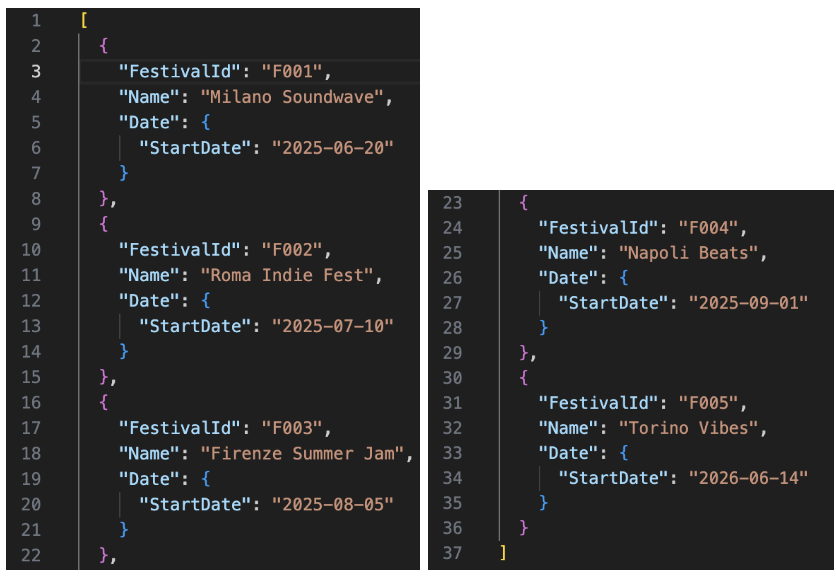
\includegraphics[width=0.7\textwidth]{R1.png}
\end{figure}
\\


\subsubsection{R2 - Festival name and drink stands only}

Description: Shows the festival name and only stands of type \texttt{"drink"}. Uses projection with:

\begin{lstlisting}
db.Festival.find(
  {},
  {
    _id: 0,
    Name: 1,
    Stands: { $elemMatch: { Type: "drink" } }
  }
).limit(3)
\end{lstlisting}

\begin{figure}[H]
    \centering
    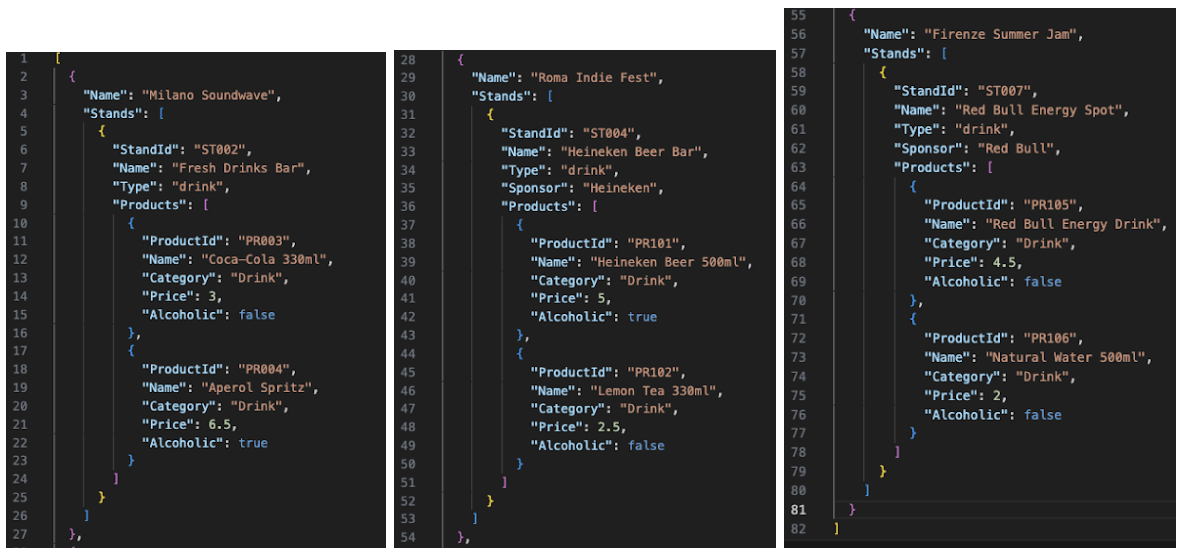
\includegraphics[width=1\textwidth]{R2.png}
\end{figure}

\subsection{Queries with limit, sort and comparison operators}
\subsubsection{R3 - Top 3 most expensive VIP tickets}

Description: Retrieves the three most expensive VIP-type tickets across all festivals. Uses comparison, \texttt{\$sort} and \texttt{\$limit}.

\begin{lstlisting}
db.Festival.aggregate([
  { $unwind: "$Tickets" },
  { 
    $match: { 
      "Tickets.Type": { $regex: "VIP" },
      "Tickets.Price": { $gt: 0 }
    } 
  },
  { $sort: { "Tickets.Price": -1 } },
  { $limit: 3 },
  {
    $project: {
      _id: 0,
      FestivalId: 1,
      FestivalName: "$Name",
      TicketType: "$Tickets.Type",
      TicketPrice: "$Tickets.Price"
    }
  }
])
\end{lstlisting}

\begin{figure}[H]
    \centering
    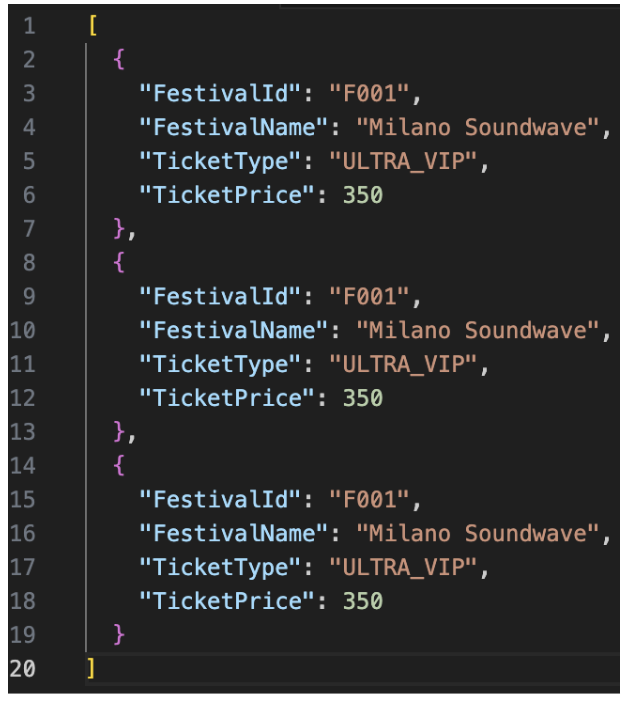
\includegraphics[width=0.5\textwidth]{R3.png}
\end{figure}

\subsubsection{R4 - First 5 festivals after 2026 ordered by start date}

Description: Returns the first five festivals starting after 1st January 2026, sorted by start date in ascending order.

\begin{lstlisting}
db.Festival.find(
  { "Date.StartDate": { $gt: "2026-01-01" } },
  {
    _id: 0,
    FestivalId: 1,
    Name: 1,
    "Date.StartDate": 1
  }
)
.sort({ "Date.StartDate": 1 })
.limit(5)
\end{lstlisting}

\begin{figure}[H]
    \centering
    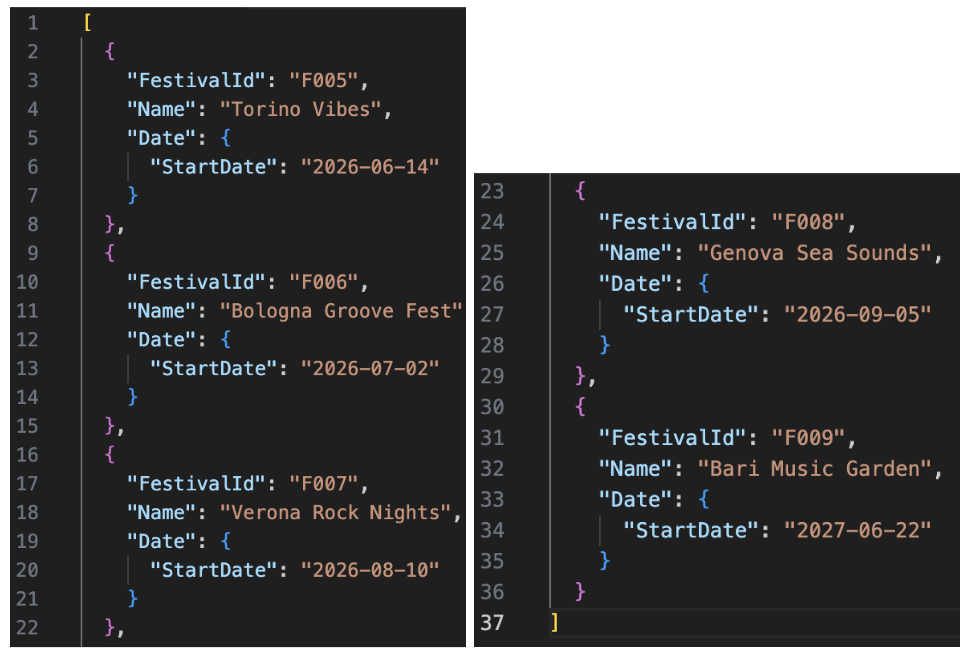
\includegraphics[width=0.7\textwidth]{R4.png}
\end{figure}

\subsection{Query including element query operators}
\subsubsection{R5 - Festivals with at least one vegetarian food product}

Description: Finds festivals that have at least one product which is a vegetarian food. Uses the element operator \texttt{\$elemMatch}.

\begin{lstlisting}
db.Festival.find(
  {
    "Stands.Products": {
      $elemMatch: { Category: "Food", IsVegetarian: true }
    }
  },
  {
    _id: 0,
    Name: 1,
    Location: 1
  }
)
\end{lstlisting}

\begin{figure}[H]
    \centering
    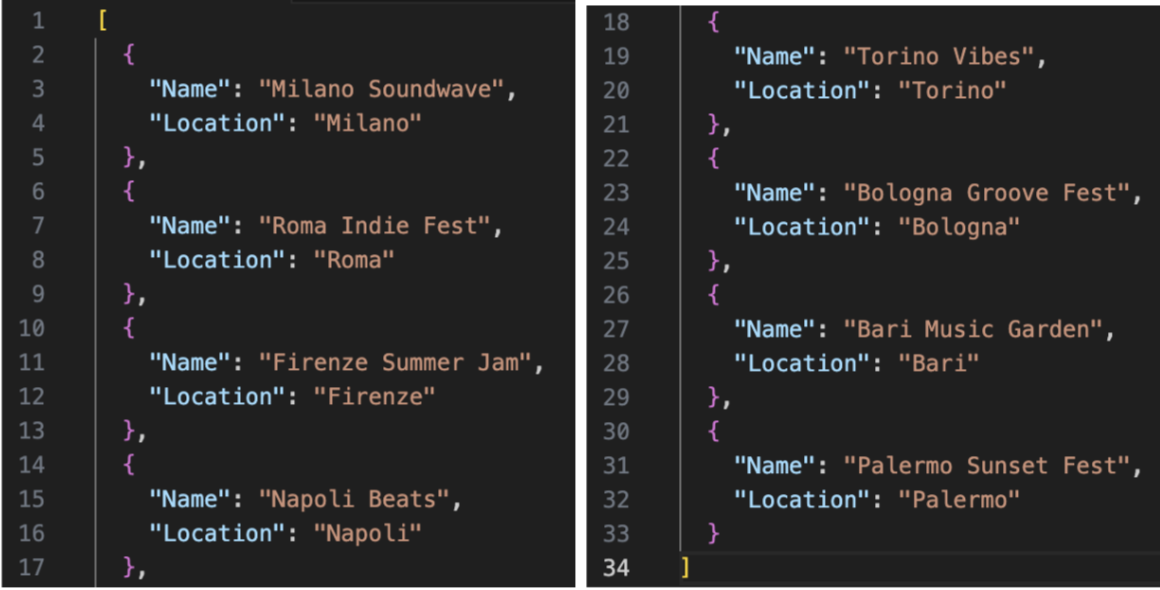
\includegraphics[width=0.7\textwidth]{R5.png}
\end{figure}

\subsection{Query using the group operator}
\subsubsection{R6 - Number of stands per festival}

Description: Counts how many stands each festival has. Uses \texttt{\$group}.

\begin{lstlisting}
db.Festival.aggregate([
  { $unwind: "$Stands" },
  {
    $group: {
      _id: "$FestivalId",
      Name: { $first: "$Name" },
      NumberOfStands: { $sum: 1 }
    }
  }
])
\end{lstlisting}

\begin{figure}[H]
    \centering
    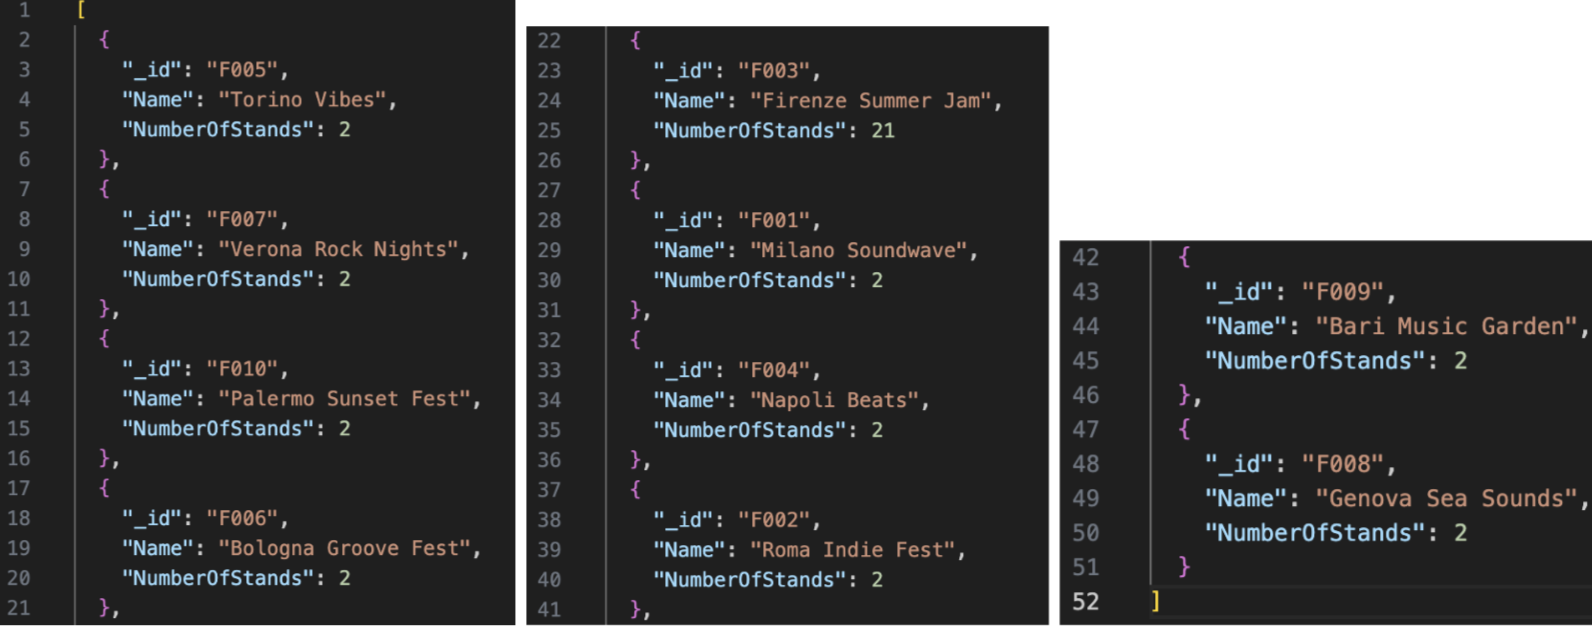
\includegraphics[width=1\textwidth]{R6.png}
\end{figure}


\subsection{Query with unwind and group by}
\subsubsection{R7 - Total performances per festival}
Description: Counts the total number of performances for each festival. Uses \texttt{\$unwind} and \texttt{\$group}.

\begin{lstlisting}
db.Festival.aggregate([
  { $unwind: "$Stages" },
  { $unwind: "$Stages.Performances" },
  {
    $group: {
      _id: "$FestivalId",
      Name: { $first: "$Name" },
      TotalPerformances: { $sum: 1 }
    }
  }
])
\end{lstlisting}

\begin{figure}[H]
    \centering
    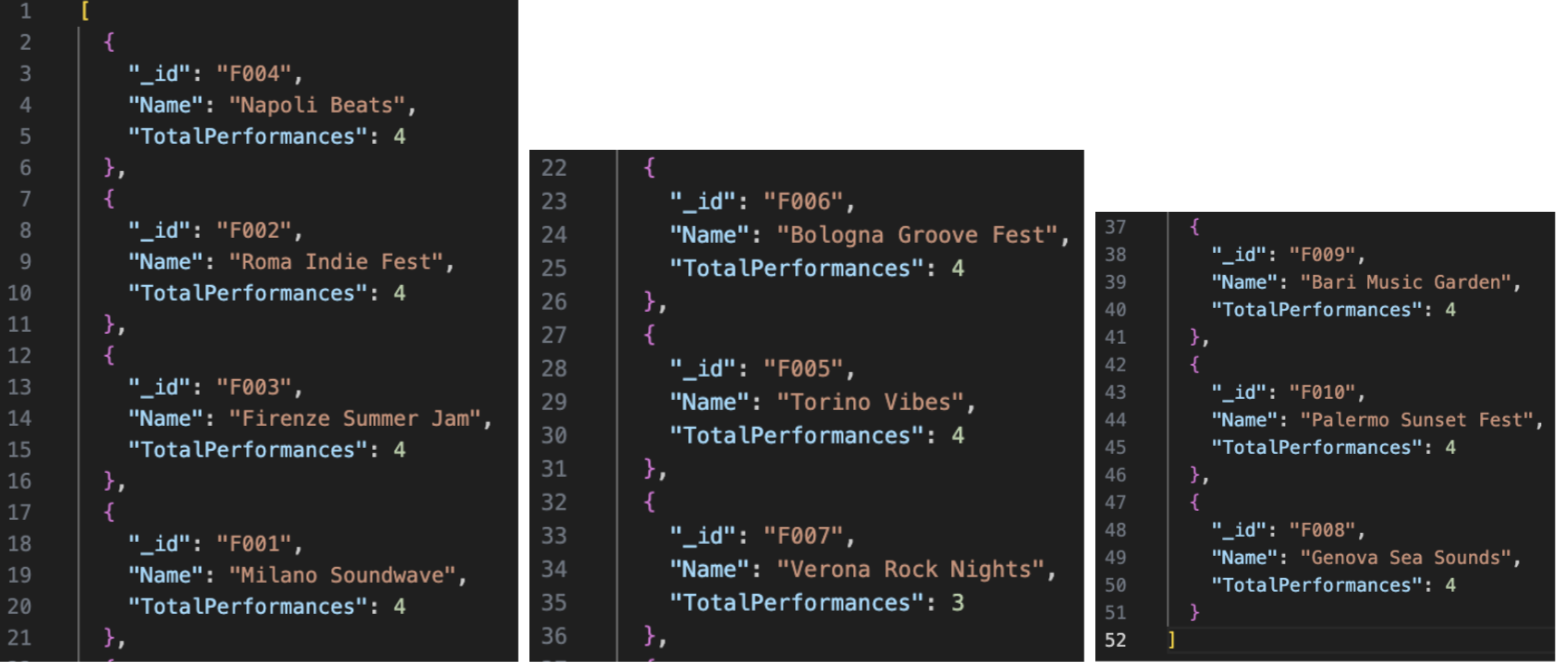
\includegraphics[width=1\textwidth]{R7.png}
\end{figure}

\subsection{Query with unwind, group by and filter}
\subsubsection{R8 - Festivals with more than 3 performances}

Description: Returns only festivals that have more than three performances in total. Uses \texttt{\$unwind}, \texttt{\$group}, then \texttt{\$match} as a filter.

\begin{lstlisting}
db.Festival.aggregate([
  { $unwind: "$Stages" },
  { $unwind: "$Stages.Performances" },
  {
    $group: {
      _id: "$FestivalId",
      Name: { $first: "$Name" },
      TotalPerformances: { $sum: 1 }
    }
  },
  {
    $match: { TotalPerformances: { $gt: 3 } }
  }
])
\end{lstlisting}

\begin{figure}[H]
    \centering
    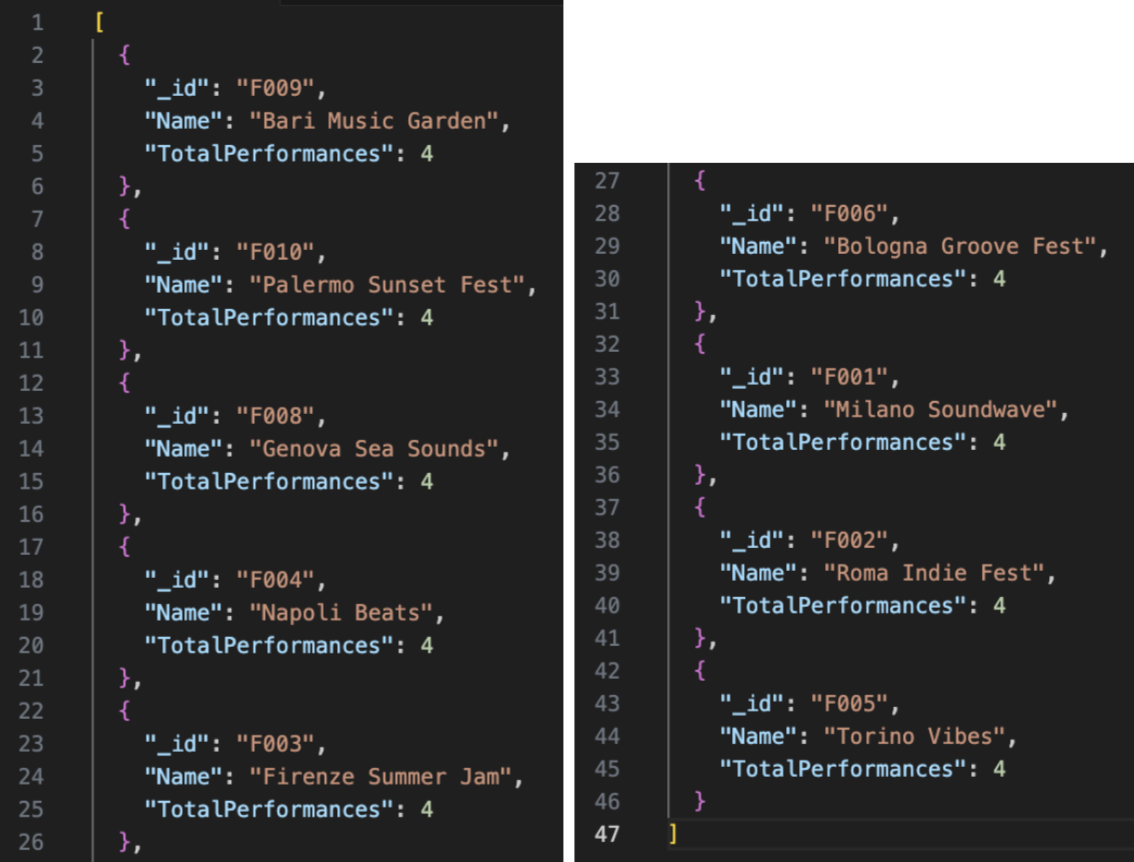
\includegraphics[width=0.7\textwidth]{R8.png}
\end{figure}

\subsection{Query with two conditions evaluated separately on the sub-documents of an array}
\subsubsection{R9 - Festivals that sell both Food and Drink products}

Description: Finds festivals that have at least one Food product and at least one Drink product, possibly in different stands or products. The two conditions are evaluated separately on different elements of the \texttt{Products} array.

\begin{lstlisting}
db.Festival.find(
  {
    $and: [
      { "Stands.Products.Category": "Food" },
      { "Stands.Products.Category": "Drink" }
    ]
  },
  {
    _id: 0,
    Name: 1,
    Location: 1
  }
).limit(5)
\end{lstlisting}

\begin{figure}[H]
    \centering
    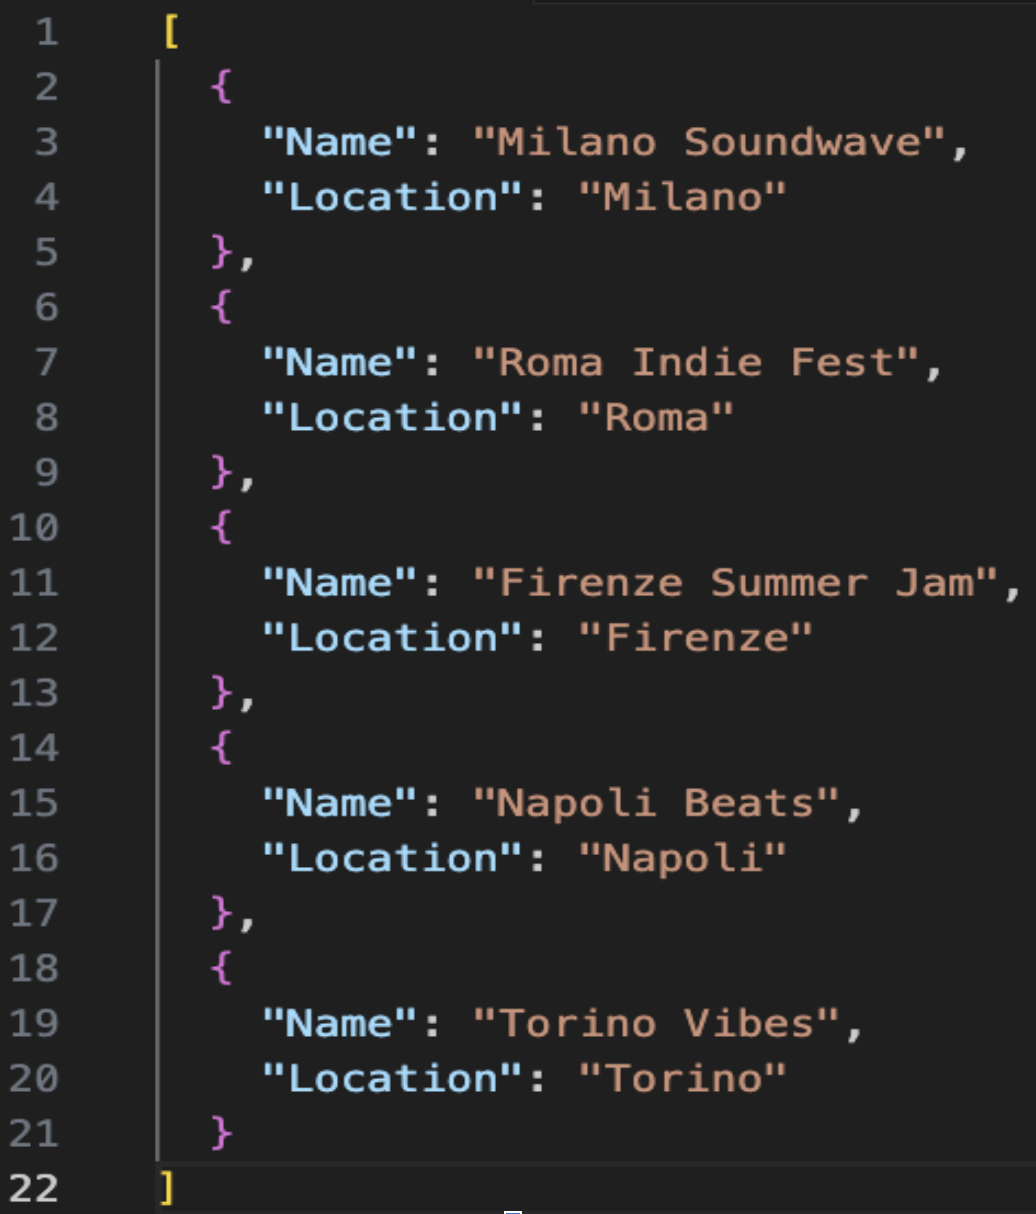
\includegraphics[width=0.5\textwidth]{R9.png}
\end{figure}

\subsection{Query with two conditions evaluated simultaneously on the sub-documents of an array}
\subsubsection{R10 - Festivals with a vegetarian food product cheaper than 7€}
Description: Finds festivals that have at least one product that is simultaneously a Food item, vegetarian, and priced below 7€. All conditions must hold for the same product. Uses \texttt{\$elemMatch}.

\begin{lstlisting}
db.Festival.find(
  {
    "Stands.Products": {
      $elemMatch: {
        Category: "Food",
        IsVegetarian: true,
        Price: { $lt: 7 }
      }
    }
  },
  {
    _id: 0,
    Name: 1,
    Location: 1
  }
).limit(5)
\end{lstlisting}

\begin{figure}[H]
    \centering
    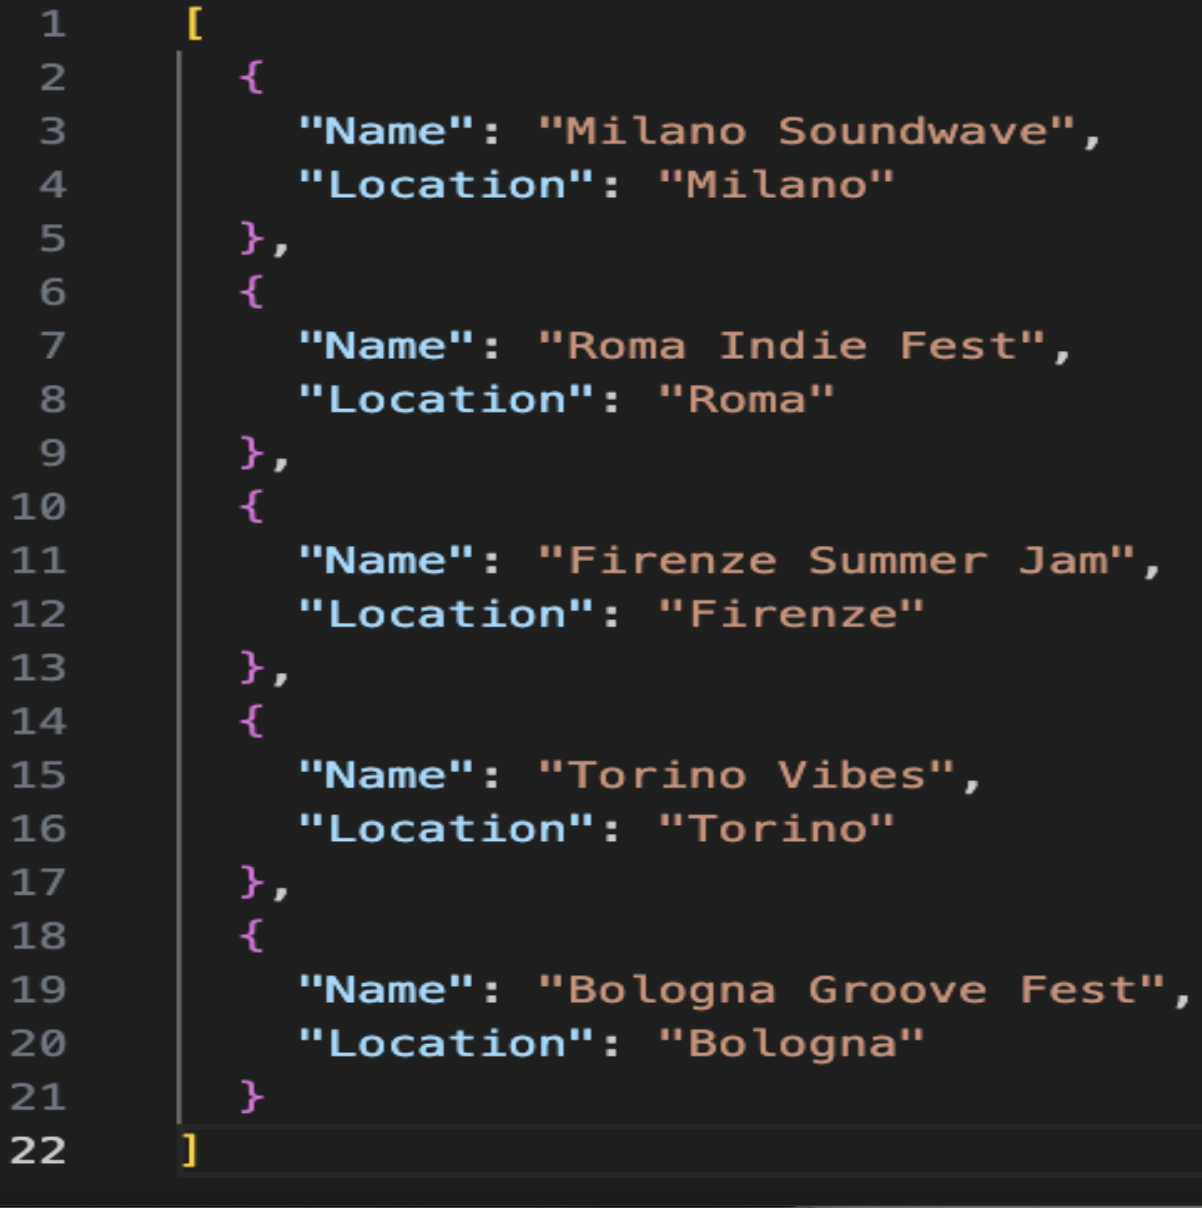
\includegraphics[width=0.5\textwidth]{R10.png}
\end{figure}

\chapter{Web}
\section{ Promotional Web Page for Euphoric Events}
This project consists of a static promotional website created for Euphoric Events.\\
The webpage promotes an instance of a fictional music festival, Milano Soundwave 2027, taking place in Parco Sempione from July 18–20, 2027.\\
The implementation uses only HTML and CSS, as required, and includes multiple sections, images, navigation links, and three additional detail pages for tickets.

\subsection{Web Page Contents and Implemented Structure}
The main page (\texttt{index.html}) is divided into major sections, each implemented with semantic HTML elements and styled through an external stylesheet.

\subsubsection{Navigation Bar}
The page begins with a \texttt{<header>} containing a logo and a \texttt{<nav>} with anchor links pointing to internal sections such as \texttt{\#hero, \#lineup, \#artists, \#stages}, and others.
 This structure allows smooth in-page navigation and separates global navigation from content.

\subsubsection{Hero Section}
The hero area \texttt{() includes}: a festival title (\texttt{<h1>}), descriptive text (\texttt{<p>}), two call-to-action buttons implemented as styled anchor tags (\texttt{<a class="btn-primary">, <a class="btn-secondary">}), and a large hero image displayed with \texttt{<img>}.\\
The section uses a two-column layout defined with CSS Grid, combining text and image.

\begin{figure}[H]
    \centering
    \includegraphics[width=0.8\textwidth]{Screenshot 2025-12-08 alle 23.55.05.png}
\end{figure}

\subsubsection{Photo Gallery}
The gallery section displays five local images (\texttt{img1.jpeg, img2.jpeg, img3.jpeg, img4.jpeg, img5.jpeg}) inside \texttt{<figure>} containers.\\
These are placed in a horizontally scrollable flex container (\texttt{.gallery-track}) with: \texttt{overflow-x: auto, scroll-snap-type: x mandatory}, hover scale and brightness \texttt{transitions ()}.\\
This creates a gallery carousel effect without using JavaScript.

\begin{figure}[H]
    \centering
    \includegraphics[width=0.8\textwidth]{Screenshot 2025-12-09 alle 00.01.17.png}
\end{figure}

\subsubsection{Line-up \& Schedule}
The line-up section organizes the festival program for all three days using: \texttt{<section>} for the block, \texttt{<article>} for each day, a subtitle, and an unordered list (\texttt{<ul><li>}) for the time and artist entries.\\
Each time label uses a \texttt{<span class="time">} to apply a distinct color and monospaced styling.\\
The list structure cleanly represents repeated performance data in readable form.

\begin{figure}[H]
    \centering
    \includegraphics[width=0.8\textwidth]{Screenshot 2025-12-09 alle 00.03.53.png}
\end{figure}

\subsubsection{Artists Section}
Artists are presented through reusable \texttt{artist card components ()}.
Each \texttt{<article class="artist-card">} contains: a \texttt{<span class="badge">} indicating Solo or Band, the artist name (\texttt{<h3>}), metadata in a \texttt{<p class="artist-meta">}, and a description paragraph.\\
The layout uses CSS Grid to produce a responsive \texttt{multi-column arrangement ()}.

\begin{figure}[H]
    \centering
    \includegraphics[width=0.8\textwidth]{Screenshot 2025-12-09 alle 00.05.28.png}
\end{figure}

\subsubsection{Stages Section}
Stages are represented using standardized card elements containing: stage name, maximum capacity, a brief description.\\
The structure again uses \texttt{<article class="card">}, maintaining visual consistency with other parts of the page.

\begin{figure}[H]
    \centering
    \includegraphics[width=0.8\textwidth]{Screenshot 2025-12-09 alle 00.06.52.png}
\end{figure}

\subsubsection{ Food, Drinks \& Merchandise}
    Three cards describe the festival’s service areas: food, drinks, and merchandise.\\
    Each card contains: a heading, a textual description, and a short unordered list of example stands, implemented through \texttt{<ul class="bullet-list">}.

\begin{figure}[H]
    \centering
    \includegraphics[width=0.8\textwidth]{Screenshot 2025-12-09 alle 00.08.19.png}
\end{figure}

\subsubsection{Tickets Section}
This section introduces three ticket types: Regular Day Pass, 3-Day Pass, VIP Experience.\\
Each ticket is displayed as a summary card with: name, price (styled via \texttt{<p class="price">}), short description, and a button linking to a dedicated page (\texttt{ticket-day.html, ticket-3day.html, ticket-vip.html}).\\
The links are standard HTML anchor tags with relative paths.
Hover effects on cards and buttons provide additional interactivity ().

\begin{figure}[H]
    \centering
    \includegraphics[width=0.8\textwidth]{Screenshot 2025-12-09 alle 00.09.50.png}
\end{figure}

\subsubsection{Ticket Detail Pages}
Three separate HTML files ( ) are used to describe each ticket type in detail.\\
Each page includes: a reused navigation bar, section title and subtitle, an overview paragraph, two structured lists (“What is included” and “Restrictions”) and a return link to the main page.
These pages reuse the same stylesheet (\texttt{style.css}), preserving design continuity.

\begin{figure}[H]
    \centering
    \includegraphics[width=0.8\textwidth]{Screenshot 2025-12-09 alle 00.11.08.png}
\end{figure}

\subsubsection{Information \& FAQ}
The final section includes logistical information (location, opening hours, permitted items).\\
The FAQ uses \texttt{<details>} and \texttt{<summary>} tags, allowing expandable panels natively without JavaScript.

\begin{figure}[H]
    \centering
    \includegraphics[width=0.8\textwidth]{Screenshot 2025-12-09 alle 00.13.15.png}
\end{figure}

\subsection{Styling and Layout (CSS)}
All styling is in \texttt{style.css ()}, which defines a consistent aesthetic and layout.

\subsubsection{Color Scheme}
The page uses a dark blue background with neon accents (cyan and fuchsia), implemented via:\\
\begin{lstlisting}
    background: radial-gradient(circle at top, #0a0f2c 0%, #05051e 100%);\\
    background: linear-gradient(135deg, #0099ff, #ff2bf0);
\end{lstlisting}

\subsubsection{Reusable Components}
CSS classes are used to create reusable UI patterns:\texttt{.card;.artist-card; .badge-solo; .badge-band; .ticket-link; .price; .tag}.
This reduces duplication and ensures consistent styling.

\subsubsection{Grid Layouts}
Multiple sections adopt CSS Grid:
\texttt{grid-template-columns: repeat(auto-fit, minmax(260px, 1fr));}
This produces responsive card grids that adapt to screen width.

\subsubsection{Hover and Transition Effects}
Cards and buttons animate through:\\
\begin{lstlisting}
transform: translateY(-6px) scale(1.03);
border-color: #00eaff;
transition: transform 0.25s ease, box-shadow 0.25s ease, border-color 0.25s ease;
\end{lstlisting}

These effects improve usability and create visual feedback.

\subsubsection{Horizontal Scrolling Gallery}
The gallery uses Flexbox and scroll snapping:\\
\begin{lstlisting}
.gallery-track {
  display: flex;
  scroll-snap-type: x mandatory;
}
\end{lstlisting}

Combined with smooth hover transitions, this creates a functional gallery without scripts.

\subsubsection{Responsive Adjustments}
Media queries refine layout on small screens:\\
\begin{lstlisting}
@media (max-width: 900px) {
  .hero-inner { grid-template-columns: 1fr; }
}
\end{lstlisting}

Navigation spacing and typography adjust accordingly.

\subsection{Conclusion}
The project uses only HTML and CSS, applying structured markup, reusable classes, grid and flex layouts, hover effects, and consistent external styling.\\
The result is a complete static website that meets the requirements for presenting a festival instance with visual clarity and organized content.
\newpage

\section{User Authentication Web Application}
This project provides a simple web interface with sign-up and log-in forms. The page sends user data to a Node.js + Express server, which validates the input and queries an SQLite database. Successful operations return a welcome message, while errors are handled both on the client and server side. The entire system is built using HTML, CSS, and a small JavaScript file.

\begin{figure}[H]
    \centering
    \includegraphics[width=0.8\textwidth]{Screenshot 2025-12-09 alle 15.25.04.png}
\end{figure}


\subsection{1. Database Design (SQLite)}
For this project we created a SQLite database named \texttt{users.db} containing a single table, \texttt{users}, designed to store all the information required for user authentication. The schema is:

\begin{lstlisting}
CREATE TABLE users (
  id INTEGER PRIMARY KEY AUTOINCREMENT,
  email TEXT UNIQUE NOT NULL,
  password TEXT NOT NULL,
  first_name TEXT NOT NULL,
  last_name TEXT NOT NULL,
  date_of_birth TEXT NOT NULL,
  address TEXT NOT NULL
);
\end{lstlisting}

This design ensures that:
\begin{itemize}
    \item the email uniquely identifies each user,
    \item passwords (stored in plain text as allowed by the assignment) can be directly compared,
    \item first name, last name, birth date and address are all required fields for registration.
\end{itemize}
To test the application, we inserted sample users:

\begin{lstlisting}
INSERT INTO users (email, password, first_name, last_name, date_of_birth, address)
VALUES 
('mario@example.com', 'MiaoPaws2025!', 'Mario', 'Rossi', '2000-05-13', 'Via Milano 10, Milano'),
('sofia@example.com', 'Ciaociao2001!', 'Sofia', 'Varotto', '2002-11-30', 'Via Roma 5, Padova)
\end{lstlisting}

\subsection{Project Files Description}
Below we provide a description of all the files included in our authentication project.
 Each file is briefly explained in terms of purpose, structure, and implemented logic.
 The full commented versions of these files are included in the submission folder.

 \subsubsection{\texttt{server.js} — Backend Logic (Node.js + Express + SQLite)}

 This file implements the entire backend of the project.  Its responsibilities include:

\textbf{1.1. Importing modules}\\
The file imports:
\begin{itemize}
    \item\texttt{express} → to create the HTTP server
    \item\texttt{sqlite3} → to query the SQLite database
    \item\texttt{path} → to locate static resources
\end{itemize}

These imports allow us to expose API routes and interact with the users.db database.

\textbf{1.2. Server and middleware initialization}\\
The server:
\begin{itemize}
    \item serves static files from \texttt{/public} using \texttt{express.static("public")}
    \item parses JSON request bodies using \texttt{express.json()}
\end{itemize}

This ensures the frontend can load correctly and send data via fetch requests.

\textbf{1.3. Database connection}\\
The SQLite database \texttt{users.db} is opened using:\\
\texttt{const db = new sqlite.Database("users.db");}\\
This allows the backend to run SQL queries for sign-up and log-in.

\textbf{1.4. Sign-Up endpoint : (POST /api/signup)}\\
This endpoint receives the data submitted by the sign-up form.\\
 The client sends all the fields required to create a new user: email, password, first\_name, last\_name, date\_of\_birth, address.\\
The server performs the following steps:

\begin{enumerate}
    \item \textbf{Server-side validation}\\
    We check that all fields are present.If any of them is missing, we immediately return:\\
    \texttt{400 Bad Request – "All fields are required."}
    \item \textbf{Safe SQL insertion}\\
    We build a parameterized SQL query:\\
    \begin{lstlisting}
    INSERT INTO users (email, password, first\_name, last\_name, date\_of\_birth, address)\\
    VALUES (?, ?, ?, ?, ?, ?)
    \end{lstlisting}
    \item \textbf{Execute Insert}\\
    We execute the query with:\\
    \texttt{db.run(sql, [...], function(err) { ... })}
    \item\textbf{Handle duplicate emails}\\
    If the email already exists, SQLite triggers: \texttt{UNIQUE constraint failed}\\
    We capture it and return: \texttt{409 Conflict – "Email already registered."}
    \item\textbf{Successful sign-up}\\
    If the user is correctly inserted, we return:\\
    \texttt{201 Created – "Welcome, FIRSTNAME! Your account has been created."}\\
    This message is displayed via \texttt{alert()} on the client side.
\end{enumerate}

\textbf{1.5 : Login endpoint  (POST /api/login)}\\
This endpoint checks whether the email and password entered by the user match a valid account. The client sends: email and password.\\
The server performs the following steps:\\

\begin{enumerate}
    \item\textbf{Validate the presence of email and password}
    If either field is empty, we immediately return:\\
    \texttt{400 Bad Request – "Email and password are required."}
    \item\textbf{Database lookup}
    We check if there is a user whose email and password match exactly:
    \begin{lstlisting}
    SELECT * FROM users\\
    WHERE email = ? AND password = ?
    \end{lstlisting}
   
\item\textbf{Handle failed login attempts}
    If no row is returned, it means: the email does not exist or the password is wrong.\\
    For security reasons, we do not distinguish between the two.\\
    We simply return: \texttt{401 Unauthorized – "Invalid email or password."}\\
    This matches real authentication systems, which never reveal which field is incorrect.
\item\textbf{Successful login}
    If a matching record is found, we return: \texttt{"Welcome back, FirstName LastName!"}\\
    The frontend shows this with an alert dialog, as required by the assignment.\\
\end{enumerate}
\textbf{1.6 Server Startup (short version)}
The following line starts the Express server on port 3000:
\begin{lstlisting}
  app.listen(3000, () => console.log("Server running on http://localhost:3000"));  
\end{lstlisting}

This makes the application accessible through the browser at \texttt{http://localhost:3000}


\subsection{Description of \texttt{index.html} and Input Requirements}

The file \texttt{index.html} defines the entire user interface of the authentication system.
 It contains two separate forms: one for user registration (sign-up) and one for authentication (log-in). The page also links the client-side script \texttt{auth.js} and the optional stylesheet \texttt{style.css}.
 
 \subsubsection{Sign-Up Form (Create a New Account)}
 The sign-up form collects all the user information required to create a new profile. Each input includes HTML5 validation rules to prevent incorrect or incomplete submissions.
 
\textbf{Email}
\begin{lstlisting}
    type="email" id="signup-email" required 
    pattern="^[^@\s]+@[^@\s]+\.[^@\s]+$" 
    title="Please enter a valid email address (example: name@mail.com)"
\end{lstlisting}

The user cannot submit the form without entering an email, it enforces a basic email format (via HTML5), we further ensure the email contains a valid domain (e.g., \texttt{.com, .it}), providing a helpful error message to the user.

\textbf{Password}
\begin{lstlisting}
    type="password"	required	
    pattern="^(?=.*[a-z])(?=.*[A-Z])(?=.*\d)(?=.*[\W_]).{8,}$"
\end{lstlisting}

We require: minimum 8 characters, at least one uppercase letter, at least one lowercase letter, at least one digit, at least one special character; to make it  similar to real websites.

\textbf{Confirm Password}\\
\texttt{type=''password  required''}\\
It must be filled, it is checked against the main password inside \texttt{auth.js} (client-side logic)

\textbf{First Name / Last Name / Address}\\
Basic text inputs 

\textbf{Date of Birth}\\
\texttt{type=''date''	required	 min=''1925-01-01''}

We ensures the user is born after 1920, preventing unrealistic ages (> 105 years old). It is a required field.


\textbf{Sign-Up Button}\\
Submits the form, but only after HTML validation succeeds.

\subsubsection{Log-In Form}
The log-in form includes only the credentials needed for authentication:
\begin{itemize}
    \item \textbf{Email}: Same validation pattern as in the sign-up form.
    \item \textbf{Password}: Basic password field; the authentication logic is handled by \texttt{auth.js} and the server.
\end{itemize}

\textbf{Log-In Button}\\
Sends the credentials to the backend via \texttt{fetch()} for verification.

The page includes the \texttt{auth.js} script using the \texttt{defer} attribute so that the JavaScript runs only after the HTML has finished loading, avoiding execution errors. It also links to \texttt{style.css}, which provides optional styling for a cleaner and more readable interface.


\subsection{auth.js}
The \texttt{auth.js} file manages the client-side logic for both user registration (sign-up) and authentication (log-in). It prevents the default form submission, validates user input, communicates with the server, and displays messages based on the server’s response.

\subsubsection{Sign-Up – Handling Success and Error Messages}
After sending the data to: \texttt{POST /api/signup},
the script waits for the server response and shows a message depending on the result.
\begin{lstlisting}
if (!response.ok) {
  alert(data.message || "Sign-up failed.");
} else {
  alert(data.message || "Sign-up successful.");
  form.reset();
}
\end{lstlisting}

The script always uses \texttt{alert()} to display the server’s message. If an error occurs, the alert shows the error text; if the registration succeeds, the alert shows the welcome message and the form is reset.

\subsubsection{Sign-Up – Network Error Message}
If the request cannot reach the server (server offline, network issue), the script shows a specific alert:
\begin{lstlisting}
.catch(() => {
  alert("Network error during sign-up.");
});
\end{lstlisting}

It shows a clear message if the browser cannot communicate with the backend at all.

\subsubsection{ Login – Handling Success and Error Messages}

When sending the credentials to: \texttt{POST /api/login},
the script shows the correct message depending on whether authentication succeeded or failed.
\begin{lstlisting}
CODE (message logic):
if (!response.ok) {
  alert(data.message || "Login failed.");
} else {
  alert(data.message || "Login successful.");
  form.reset();
}
\end{lstlisting}

If the credentials are wrong, the script shows the error message through \texttt{alert()}. If the login succeeds, it displays the welcome message with \texttt{alert()} and resets the form.

\subsection{Login – Network Error Message}

If the login request cannot reach the server:\\
\textbf{CODE (network error):}\\
\texttt{.catch(() => { alert("Network error during login."); });}

Ensures that even in case of connection problems, the user receives a clear, understandable alert.

\subsection{style.css}
This CSS file applies simple styling to improve readability and layout. It sets a clean font, adds spacing around forms and inputs, styles labels and buttons for better usability, and provides a hover effect on the submit button. Overall, it keeps the interface minimal and consistent.

\end{document}
